\section{Valve Closing Simulations} \label{sec: ClosingSimulation}

Now the dynamics of the system of dimensionless differential equations, \cref{eq: Non-DimODE}, will be studied using numerical simulations. This is done using the MATLAB in-built function \textit{ode45}, which uses a 4th order Runge-Kutta method with a 5th order Runge-Kutta corrector to minimise error~\cite{Shampine1997TheSuite}. The simulation of when the valve is slightly perturbed from the equilibria in the negative $x$ direction is shown in \cref{fig:TimeTrajec}. As predicted from the stability analysis, the perturbation grows exponentially until it reaches the low valve stop. At this point, a series of collisions occur which are modelled by considering the impact law given in \cref{sec: ValveCollision}. The collision is implemented by stopping the simulation when one occurs, and using the current values for $x$, $p_t$ and $\dot{x}^+$ from the impact law to form the initial conditions to restart the simulation.
~
\begin{figure}[!ht]
    \centering
    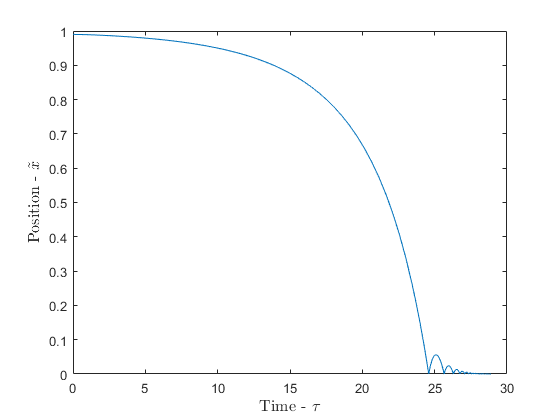
\includegraphics[width=0.7\textwidth]{Figures/Example/PositionTimeTrajectory.png}
    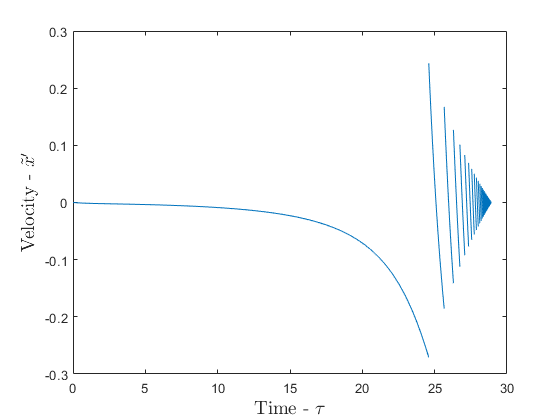
\includegraphics[width=0.49\textwidth]{Figures/Example/VelocityTimeTrajectory.png}
    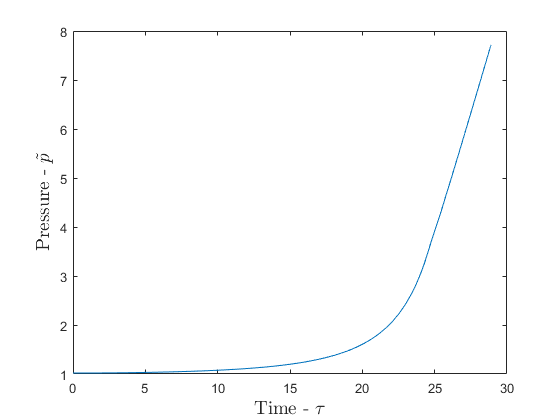
\includegraphics[width=0.49\textwidth]{Figures/Example/PressureTimeTrajectory.png}
    \caption{Simulation results for $\alpha = 0.1$ and $\beta = 1$.}
    \label{fig:TimeTrajec}
\end{figure}

The dynamics in \cref{fig:TimeTrajec} show the desired behaviour in which the valve closes. Interestingly, the valve requires a series of impacts to gradually decrease the velocity until the valve is at rest. However, these impacts do not constitute a chatter instability, as they are low frequency and non-sustained. With these impacts, the valve will close in a finite time, which will be discussed later in this report%, \cref{sec:ValveCloseImpacts} 
.

Although the valve position and velocity both tend towards zero, the tank pressure does not show similar behaviour as instead $p_t \rightarrow \infty$. This may initially seem slightly counter-intuitive except for two important restrictions of this simple model. Firstly, the pilot valve is completely ignored, which means the main valve will never open once it has closed as the opening mechanism is dependent on the pilot valve. Secondly, except in the limit that $\alpha \rightarrow 0$ and $\beta \rightarrow \infty$, there is also a non-zero mass flow rate into the tank, or equivalently $\dot{m}_{in} \neq 0$. Hence, when the valve is closed, the mass of fluid is still increasing. Therefore, the density must slightly increase so the pressure must also slightly increase.

% % Example Trajectory in Phase Portrait - PROBABLY NOT WORTH USING
% \begin{figure}[!ht]
%     \centering
%     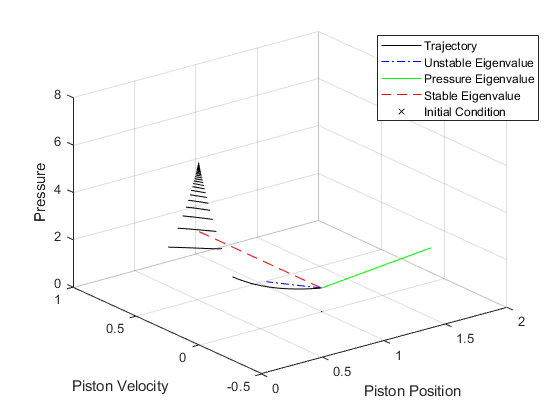
\includegraphics[width=0.49\textwidth]{Figures/Example/PhasePotrait3D.png}
%     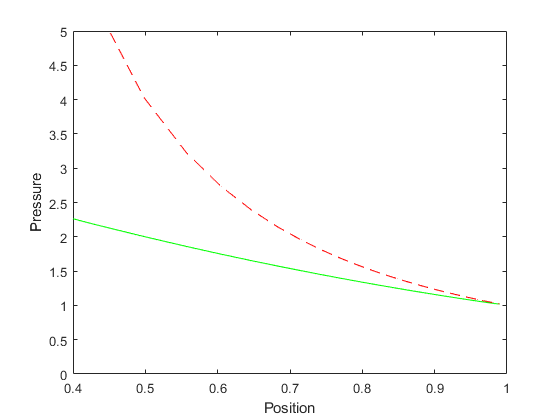
\includegraphics[width=0.49\textwidth]{Figures/Example/PressurePositionPhasePotrait2D.png}
%     \caption{Caption}
%     \label{fig:ExamplePhase}
% \end{figure}

% % Example Trajectory in eigenvector projected Phase Portrait - DO NOT USE
% \begin{figure}[!ht]
%     \centering
%     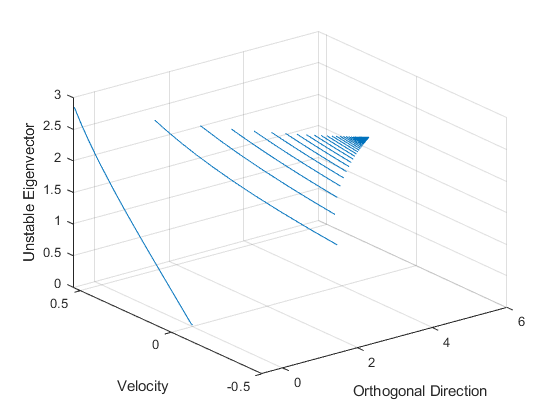
\includegraphics[width=0.7\textwidth]{Figures/Example/EigenvectorPhasePotrait3D.png}
%     \caption{Caption}
%     \label{fig:EigPhase}
% \end{figure}

% % Example Trajectory of eigenvector space in 2D Phase and 1D unstable trajectory - DO NOT USE
% \begin{figure}[!ht]
%     \centering
%     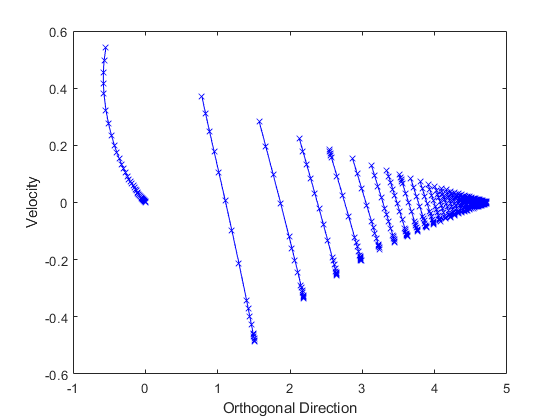
\includegraphics[width=0.49\textwidth]{Figures/Example/PhasePotrait2D.png}
%     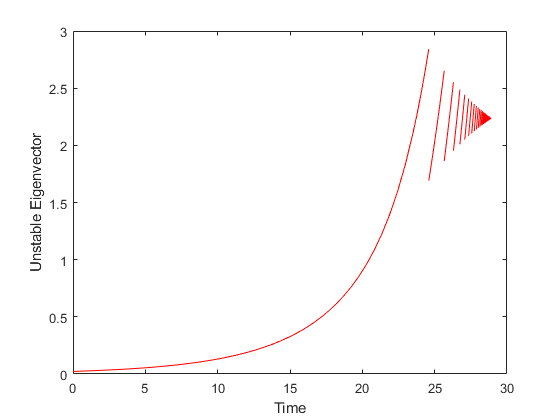
\includegraphics[width=0.49\textwidth]{Figures/Example/UnstableEigenvectorTrajectory.png}
%     \caption{Caption}
%     \label{fig:EigenvectorPhase}
% \end{figure}

\section{Low flow rates}

As has been previously identified, for low flow rates were $\dot{m}_{in} \rightarrow 0$, the limit of $\alpha \rightarrow 0$ and $\beta \rightarrow \infty$ occurs. Focusing on only the limit of $\alpha \rightarrow 0$, the eigenvalues of the linearised form of \cref{eq: Non-DimODE} around the equilibrium are
~ % eigenvalues
\begin{equation*}
    \lambda_1 = - \frac{1}{2}\beta \, , \quad
    \lambda_2 = -1 \, , \quad
    \lambda_3 = 0 \, .
\end{equation*}

Similarly, the eigenvectors in the limit of $\alpha \rightarrow 0$ are
~ % eigenvectors
\begin{equation*}
    v_1 = \begin{pmatrix}
    0 & 0 & 1
    \end{pmatrix}^T \qquad
    v_2 = \begin{pmatrix}
    \frac{2 - \beta}{2\beta} & \frac{\beta - 2}{2\beta} & 1
    \end{pmatrix}^T \qquad
    v_3 = \begin{pmatrix}
    - \frac{1}{2} & 0 & 1
    \end{pmatrix}^T \, .
\end{equation*}

This reveals several interesting results about a low flow rate scenario. Firstly, the equilibrium becomes neutrally stable. This is particularly interesting as it suggests that if there is no mass flow into the tank, the main valve will not close. However, this represents the case for which the tank equilibrium pressure is $p_t = 0$. In this case, the main piston obviously will not move as there are no fluid forces acting upon the main piston.

There is also one constant eigenvalue, $\lambda_2$, which does not depend upon $\beta$. In the limit that $\beta \rightarrow \infty$, the corresponding eigenvector is $v_2 = \left( - \frac{1}{2}, \frac{1}{2}, 1 \right)^T$. This is the only eigenvector with a component in  the velocity direction, which suggests that for sufficiently large $\beta$, the dynamics in the velocity component are near identical. \Cref{fig: ValveClose3DPhase} shows the phase portrait in position-velocity-pressure space, which shows very similar behaviour in the velocity direction for two different $\beta$ values.
~
% The three dimensional phase portrait in Position-Velocity-Pressure phase space can be seen below.
% 
\begin{figure}[ht]
    \centering
    \begin{subfigure}{0.49\textwidth}
    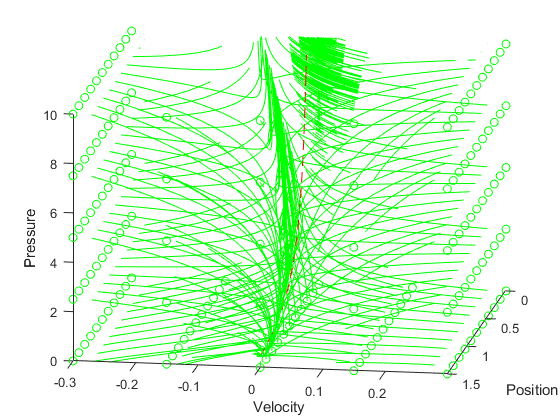
\includegraphics[width=\textwidth]{Figures/LowFlow/3DPhase-b=1.png}
    \caption{$\alpha = 0.01, \, \beta = 1$}
%    \label{fig:1}
    \end{subfigure}
    \begin{subfigure}{0.49\textwidth}
    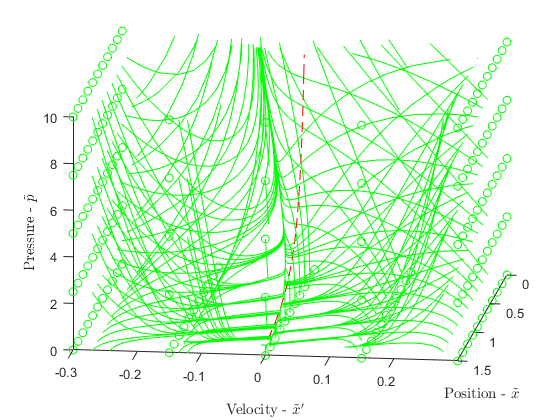
\includegraphics[width=\textwidth]{Figures/LowFlow/3DPhase-b=10.png}
    \caption{$\alpha = 0.01, \, \beta = 10$}
%    \label{fig:2}
    \end{subfigure}
    \caption{3D Phase Portrait}
    \label{fig: ValveClose3DPhase}
\end{figure}

In fact, we see that the dynamics approaches the unstable manifold of the equilibrium. The valve then either follows the manifold in the direction of decreasing piston position, so that the valve closes. Alternatively, the dynamics follow the manifold with increasing valve position, so that the valve closes. Regardless of the value of $\beta$ used, the unstable manifold appears to have an identical shape in the velocity dimension. Because of the similar behaviour in the velocity direction, phase portraits will now only show a 2D representation in the position-pressure space for clarity.

One difference which can be seen between the phase portraits for $\beta = 1$ and $\beta = 10$, \cref{fig: ValveClose3DPhase}, is due to impact dynamics. For $\beta = 1$, the valve collides with the lower stop at a low enough pressure that it can be seen in the pressure range shown in \cref{fig: ValveClose3DPhase}. These dynamics are predictable in that an impact occurs so the velocity reverses, but the piston is still being forced downwards by the fluid. Hence, the impacts continue while the velocity tends to 0. This will be further explored in \cref{sec: ImpactDynamics}.

By looking at \cref{eq: Non-DimODE}, we see that as $\alpha \rightarrow 0$ and $\beta \rightarrow \infty$, a slow-fast system occurs. Hence, we expect the dynamics to quickly approach the equilibrium pressure, so that
~
\begin{equation*}
    1 - \tilde{x} \sqrt{\tilde{p}} = 0 \, .
\end{equation*}

This is in agreement with the eigenvalues, as $\lambda_1 \rightarrow - \infty$. The corresponding eigenvector, $v_1$, shows these dynamics purely effect the tank pressure locally to the equilibrium. In fact, this is exactly what we see in \cref{fig: ValveClose3DPhase}, where the vertical lines show the dynamics very quickly approach the equilibrium pressure. In fact, the dynamics approach the family of equilibria which exist as $\dot{m}_{in} \rightarrow 0$. Further from the equilibrium at $\tilde{x} = 1$, the fast dynamics do not act purely horizontally.
~
% The phase portrait in Position-Pressure space can be seen below
% 
\begin{figure}[ht]
    \centering
    \begin{subfigure}{0.49\textwidth}
    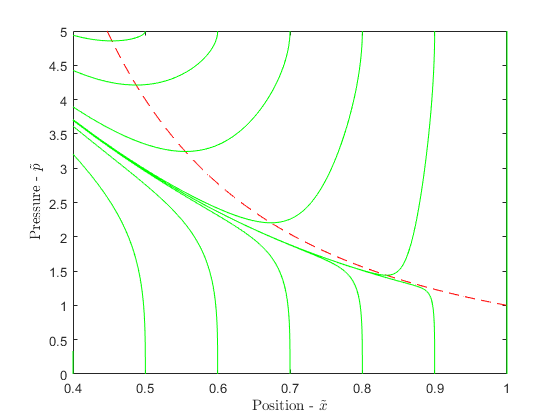
\includegraphics[width=\textwidth]{Figures/LowFlow/PhasePortrait-b=1.png}
    \caption{$\alpha = 0.01, \, \beta = 1$}
    \label{fig: ValveClosePhase1}
    \end{subfigure}
    \begin{subfigure}{0.49\textwidth}
    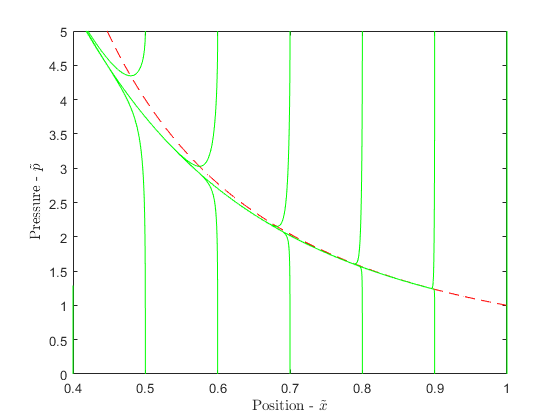
\includegraphics[width=\textwidth]{Figures/LowFlow/PhasePortrait-b=10.png}
    \caption{$\alpha = 0.01, \, \beta = 10$}
    \label{fig: ValveClosePhase10}
    \end{subfigure}
    \caption{2D Phase Portrait}    \label{fig: ValveClosePhase}
\end{figure}

In fact, as $\alpha \rightarrow 0$ and $\beta \gg 1$, the equation $1 - \tilde{x} \sqrt{\tilde{p}} = 0$ gives a closer approximation to the unstable manifold. However, even when $\beta$ is not sufficiently large, this gives a good approximation sufficiently close to the equilibrium. This expression is tangeant to the unstable eigenvector given by $v_3$ at the equilibrium.

% Simulation results support this. 
% 
% % 2D Phase Portrait showing low flow rate trajectory close to manifold - PROBABLY DO NOT (TOO SIMILAR TO BELOW)
% \begin{figure}[ht]
%     \centering
%     \begin{subfigure}{0.49\textwidth}
%     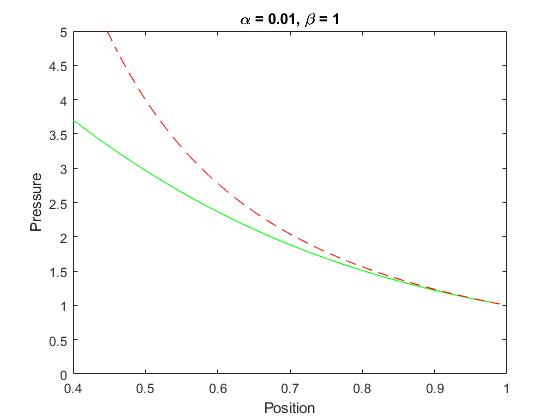
\includegraphics[width=\textwidth]{Figures/LowFlow/b=1.png}
%     \caption{$\alpha = 0.01, \, \beta = 1$}
% %    \label{fig:1}
%     \end{subfigure}
%     \begin{subfigure}{0.49\textwidth}
%     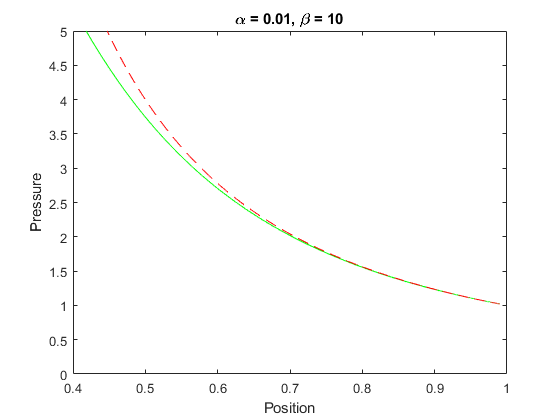
\includegraphics[width=\textwidth]{Figures/LowFlow/b=10.png}
%     \caption{$\alpha = 0.01, \, \beta = 10$}
% %    \label{fig:2}
%     \end{subfigure}
% %    \label{3}
% %    \caption{}
% \end{figure}

%\newpage
\section{Fixed Tank Pressure}

One interesting case is when the mass flow rate into the tank, $\dot{m}_{in}$, is allowed to vary such that the tank pressure remains constant. As both $\alpha$ and $\beta$ are functions of $\dot{m}_{in}$ in \cref{eq: Non-DimODE}, this set of dimensionless equations is not useful for the purpose of constant tank pressure. Instead, a new set of dimensionless equations will be introduced. These use the valve equilibrium lift as the reference distance and ambient pressure as the reference pressure.

Hence, the reference dimensions are given by
~
\begin{equation*}
\begin{split}
    x_{ref} = \frac{1}{C_d} \sqrt{\frac{A_v - A_p}{4 \pi}}
    \, , \qquad
    p_{ref} = p_a = 1 \si{bar}
    \, , \qquad
    \omega_{ref} = C_d \sqrt{4 \pi} \sqrt{\frac{p_{ref} x_{ref}}{m_v}} \, .
\end{split}
\end{equation*}

Using these reference dimensions, the dimensionless set of differential equations are given by
~
\begin{equation} \label{eq: AltNonDim}
\begin{split}
    \ddash{\tilde{x}} + \kappa \, \dash{\tilde{x}} &=  \tilde{p} \left( \tilde{x}\power{2}  - 1 \right) \, , \\
    \dash{\tilde{p}} &= \beta \left( q - \sigma \mu \, \tilde{x} \, \sqrt{\tilde{p}} \right) \, .
\end{split}
\end{equation}

This system of equation uses significantly more dimensionless parameters than \cref{eq: Non-DimODE}. However, \cref{eq: AltNonDim} uses dimensionless parameters which are consistent with those used later in this report in \cref{subsec: QWMNonDim}. One important parameter is $q$, which represents the flow into the tank is expressed in terms of the fraction of the maximum flow allowable, a fixed constant $\dot{m}_{cap}$. The definition of all the dimensionless parameters used are
~
\begin{equation*}
    \begin{tabular}{p{2.1cm} p{2.8cm} p{2.1cm} p{3cm} p{2.8cm}}
        $ \kappa = \frac{c_v}{m_v \omega_{ref}} \, , $
        &
        $ \beta = \frac{a^2}{V} \frac{\dot{m}_{cap}}{p_{ref} \omega_{ref}} \, , $
        &
        $ q = \frac{\dot{m}_{in}}{\dot{m}_{cap}} \, , $
        &
        $ \mu = \frac{\rho A_p \omega_{ref} x_{ref}}{\dot{m}_{cap}} \, , $
        &
        $ \sigma = \frac{\zeta x_{ref} \sqrt{\rho p_{ref}}}{A_p \rho x_{ref} \omega_{ref}} \, . $
    \end{tabular}
\end{equation*}

It is now clear why such a non-dimensionalisation was chosen. For the tank pressure to be constant, either $\beta = 0$ or the mass inflow to the tank matches that discharge through the main valve exactly. For the case that $\beta \neq 0$, the mass flow into the tank must satisfy
~
\begin{equation*}
    q = \sigma \mu \, \tilde{x} \, \sqrt{\tilde{p}} \, .
\end{equation*}

Now, the tank pressure $\tilde{p}$ is a fixed parameter that the tank is held at. Hence, the mass flow into the tank must be directly proportional to the valve lift.
~
% POSSIBLY INCLUDE TWO GRAPHS OF $\tilde{x}$ AND $q$?! MAYBE SET MAXIMUM OF $q = 1$ AND SHOW PRESSURE AS VALVE CLOSING
% 
\begin{figure}[!ht]
    \centering
    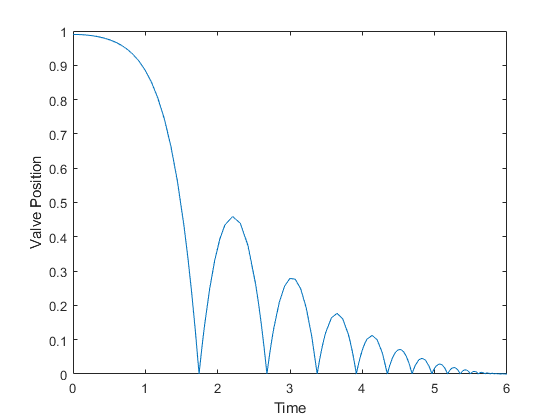
\includegraphics[width=0.49\textwidth]{Figures/FixedPressure/Position.png}
    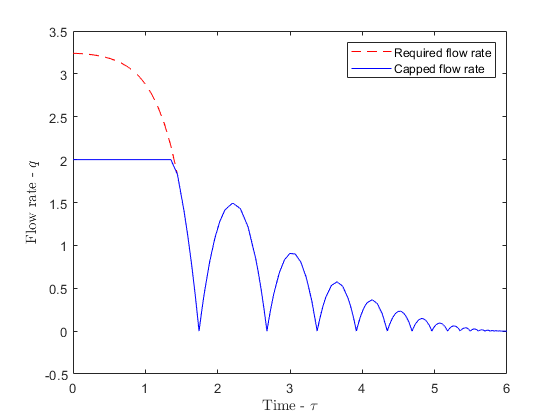
\includegraphics[width=0.49\textwidth]{Figures/FixedPressure/FlowRate.png}
    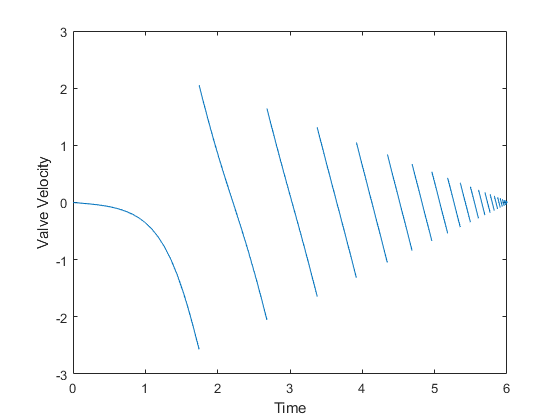
\includegraphics[width=0.49\textwidth]{Figures/FixedPressure/Velocity.png}
    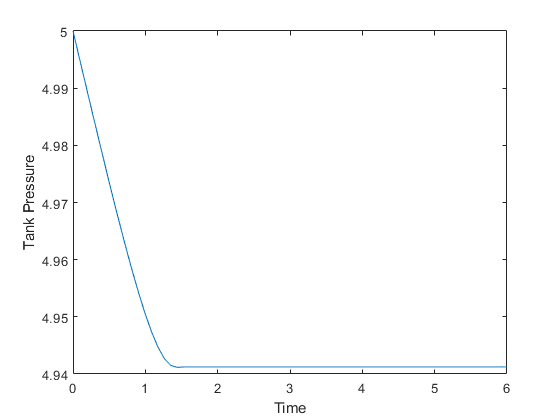
\includegraphics[width=0.49\textwidth]{Figures/FixedPressure/Pressure.png}
    \caption{Simulation when maximum flow rate into the tank is $q = 2$}
    \label{fig: FixPres}
\end{figure}

\textcolor{Red}{WRITE A PARAGRAPH ABOUT THIS GRAPH TO FINISH SECTION!}

\newpage
\section{Impact Dynamics} \label{sec: ImpactDynamics}

Now some more thorough consideration of the collisions with either the upper or lower stop will be considered. This is of particular use to simulate the dynamics of the valve between the first collision with the lower stop until the valve remains fully closed. Hence, if the pilot valve dynamics are also considered, a simulation would be able to reproduce the valve closing and then re-opening which is useful to study if cycling may occur. \Cref{fig: ImpactPos} shows the simulation of typical dynamics for a collision with the upper stop. The following analysis can be repeated for a collision with the lower stop, however this is almost identical so will not be considered.
~
\begin{figure}[ht]
    \centering
    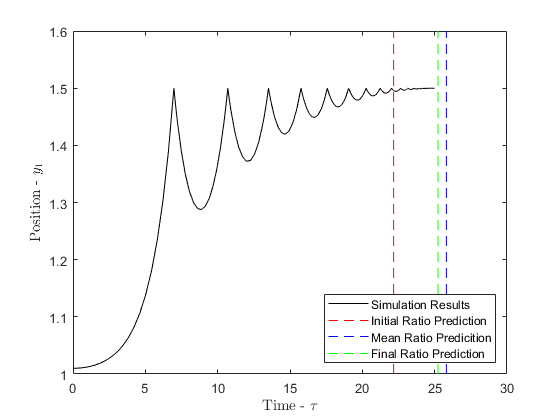
\includegraphics[width=0.7\textwidth]{Figures/ImpactSeries/PositionTime.png}
    \caption{Predictions of valve closing time using different calculated ratios.}
    \label{fig: ImpactPos}
\end{figure}

The important feature to notice is that the time between each successive impact seems to decrease, leading to a series of very small impacts which occur more frequently. We can consider the time between the $i$-th impact and the next impact a converging series. Hence, each term in this series may be written as
~
\begin{equation*}
    T_i = t_{i+1} - t_{i} \, ,
\end{equation*}

where $t_i$ represents the time at which the $i$-th impact occurs.

An important use of this series is to calculate the time at which the final impact occurs, at which point the valve remains closed. This is given by $t_\infty$, however this would involve an infinite number of collisions which is not feasible for simulation. However, the time at which the valve remains closed, $t_f$, may be expressed as
~
\begin{equation*}
    t_f = t_\infty = t_1 + \sum^\infty_{i = 1} T_i \, .
\end{equation*}

Now we must find if the series is a geometric series for which a common ratio $r$ exists and is constant for all terms, such that $T_i = T_0 \cdot r^i$ and each successive term is the previous term multiplied by the common ratio. \Cref{fig: ImpactOtherRatio} shows how the ratio between successive terms of $T_i$ changes as more impacts occur. It can be seen that this common ratio $r$ is nearly constant over all impacts, however some small variation does exist.

\newpage
If the initial common ratio, i.e. $r = \sfrac{T_2}{T_1}$, is used to predict the closing time assuming the time between collisions follows a geometric series, the time at which the valve finally closes is greatly underestimated. This can be seen in \cref{fig: ImpactPos} where the red vertical dashed line represents the time at which the valve is predicted to be fully closed. Clearly, the simulated oscillations occur past this point. This is expected from \cref{fig: ImpactOtherRatio}, where the initial common ratio is much lower than the future ratios.
~
\begin{figure}[ht]
    \centering
    \begin{subfigure}{0.49\textwidth}
    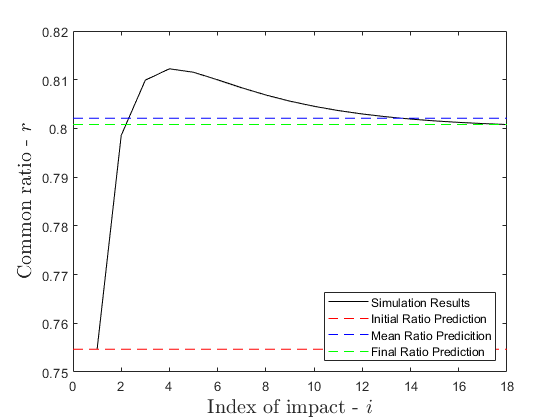
\includegraphics[width=\textwidth]{Figures/ImpactSeries/CommonRatio.png}
    \caption{Common ratio between impacts.}
    \label{fig: ImpactOtherRatio}
    \end{subfigure}
    \begin{subfigure}{0.49\textwidth}
    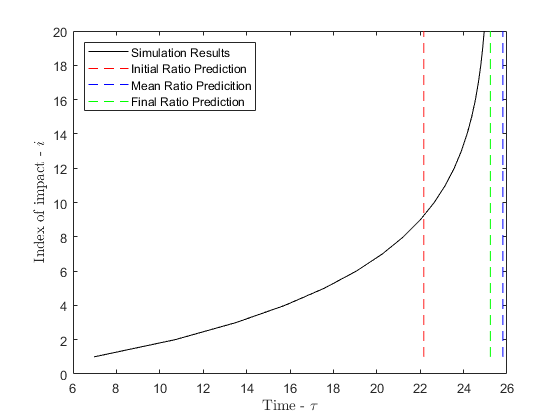
\includegraphics[width=\textwidth]{Figures/ImpactSeries/FinalTime.png}
    \caption{Time of each successive impact.}
    \label{fig: ImpactOtherTimes}
    \end{subfigure}
    \caption{Ratio between time of each impact occurring and the time of each impact.}
    \label{fig: ImpactOther}
\end{figure}

Now we consider the case for which the simulation has modelled the collisions until numerical errors prevent further simulation. It can be seen from \cref{fig: ImpactOtherRatio} that the common ratio $r$ does eventually tend towards a constant value. This means as the collisions continue to occur, the time between each impact appears to tends towards a geometric series. 

So two alternative approximations of the common ratio are used to predict the valve closing time. The first is to simply take the mean average of the common ratios. The second is to consider the geometric series only occurs continues after the collisions can no longer be simulated, such that the last calculated common ratio is used.%, such that $r = \sfrac{T_N}{T_{N-1}}$.
When these common ratios are calculated, it can be seen in \cref{fig: ImpactOtherRatio} that both give similar values for $r$.

From \Cref{fig: ImpactPos}, it is clear both of these approaches give a reasonable estimate of when the final collision occurs and the valve remains closed. However, \cref{fig: ImpactOtherTimes} shows how the time at which each collision occurs. It appears using the final common ratio gives the better approximation of the finite time of the collision when $i \rightarrow \infty$. Hence, to calculate the time at which the valve remains closed, the best approximation is given by
~
\begin{equation*}
\begin{split}
    a = T_{N-2} \, , \qquad %= t_{N-1} - t_{N-2} \\
    r = \frac{T_{N-1}}{T_{N-2}} \, , \qquad %= \frac{t_N - t_{N-1}}{t_{N-1} - t_{N-2}} \\
    t_f = t_{N-2} + \frac{a}{1-r} \, ,
\end{split}
\end{equation*}

where $i = N$ is the index of the final collision which has been simulated. This may be written in terms of the time of each collision, such that

\begin{equation*}
    t_f = t_{N-2} + \frac{\left( t_{N-1} - t_{N-2} \right)^2}{2 \, t_{N-1} - t_N - t_{N-2}} \, .
\end{equation*}